\documentclass[11pt]{article}

\usepackage[T1]{fontenc}
\usepackage{librefranklin}
\renewcommand*\familydefault{\sfdefault} %% Only if the base font of the document is to be sans serif

% \author{Nikolas Eptaminitakis}
\date{}
\usepackage{mymacros}

\begin{document}

\section*{Ecological Models Worksheet}


\subsection*{Predator-Prey Systems}
Our goal is to model two species, one of which (the predator) feeds on the other (the prey). The prey feeds on some third food item in the environment.
We denote the population of the prey as a function of time by $x(t)$ and the one of the predator by $y(t)$.
% If you took MA 266, for one of the computer projects you had to study a population of ladybugs (predators) interacting with a population of aphids (prey).
An example is foxes preying on rabbits; the latter feed on vegetation.
The assumptions of the model are the following:
\begin{enumerate}
	\item In the absence of predators, the prey population grows at natural rate $\frac{dx}{dt}=ax$, $a>0$
	\item In the absence of prey, the population of predators declines  at natural rate, $\frac{dy}{dt}=-by$, $b>0$
	\item Encounters between predators and prey result in an increase of the growth rate of predators which is proportional to the product $xy$ and a decrease of the growth rate of the prey which is also proportional to $xy$.
\end{enumerate}
We have the general \textbf{predator-prey system}
\begin{equation}
	\begin{aligned}
		&\frac{dx}{dt}=ax-pxy = x(a-py)\\	
		&\frac{dy}{dt}=-by+qxy=y(-b+qx)
	\end{aligned}
		% 
\end{equation}
with $a,b,p,q>0$.
Notice where the signs are! It is the signs that make $x$ stand for the population of a prey and $y$ the population of a predator.

\begin{example}
	Suppose you are given the following predator-prey system describing a population of foxes and rabbits in a large forest.
	\begin{equation}\label{predator-prey}
	\begin{aligned}
		&\frac{dx}{dt}=200x-4xy \\	
		&\frac{dy}{dt}=-150y+2xy
	\end{aligned}
		% 
\end{equation}
\end{example}

\begin{enumerate}
	\item Which of the two variables $x$, $y$ corresponds to the foxes and which one to the rabbits?
	\item Find the critical points of the system \eqref{predator-prey}.
	\item At each of the critical points, compute the linearzation of the system and the eigenvalues of the linearized systems. 
	What does the phase plane portrait look like for each of the linearized systems (node, spiral, center etc)? Describe their stability.
	\item What can you say about the type and stability of each critical point of the nonlinear system \eqref{predator-prey}?
	\item \label{4} Which of the options below corresponds to the phase plane portrait of the nonlinear system \eqref{predator-prey}?

	\begin{figure}[h]
		\minipage{0.32\textwidth}
		  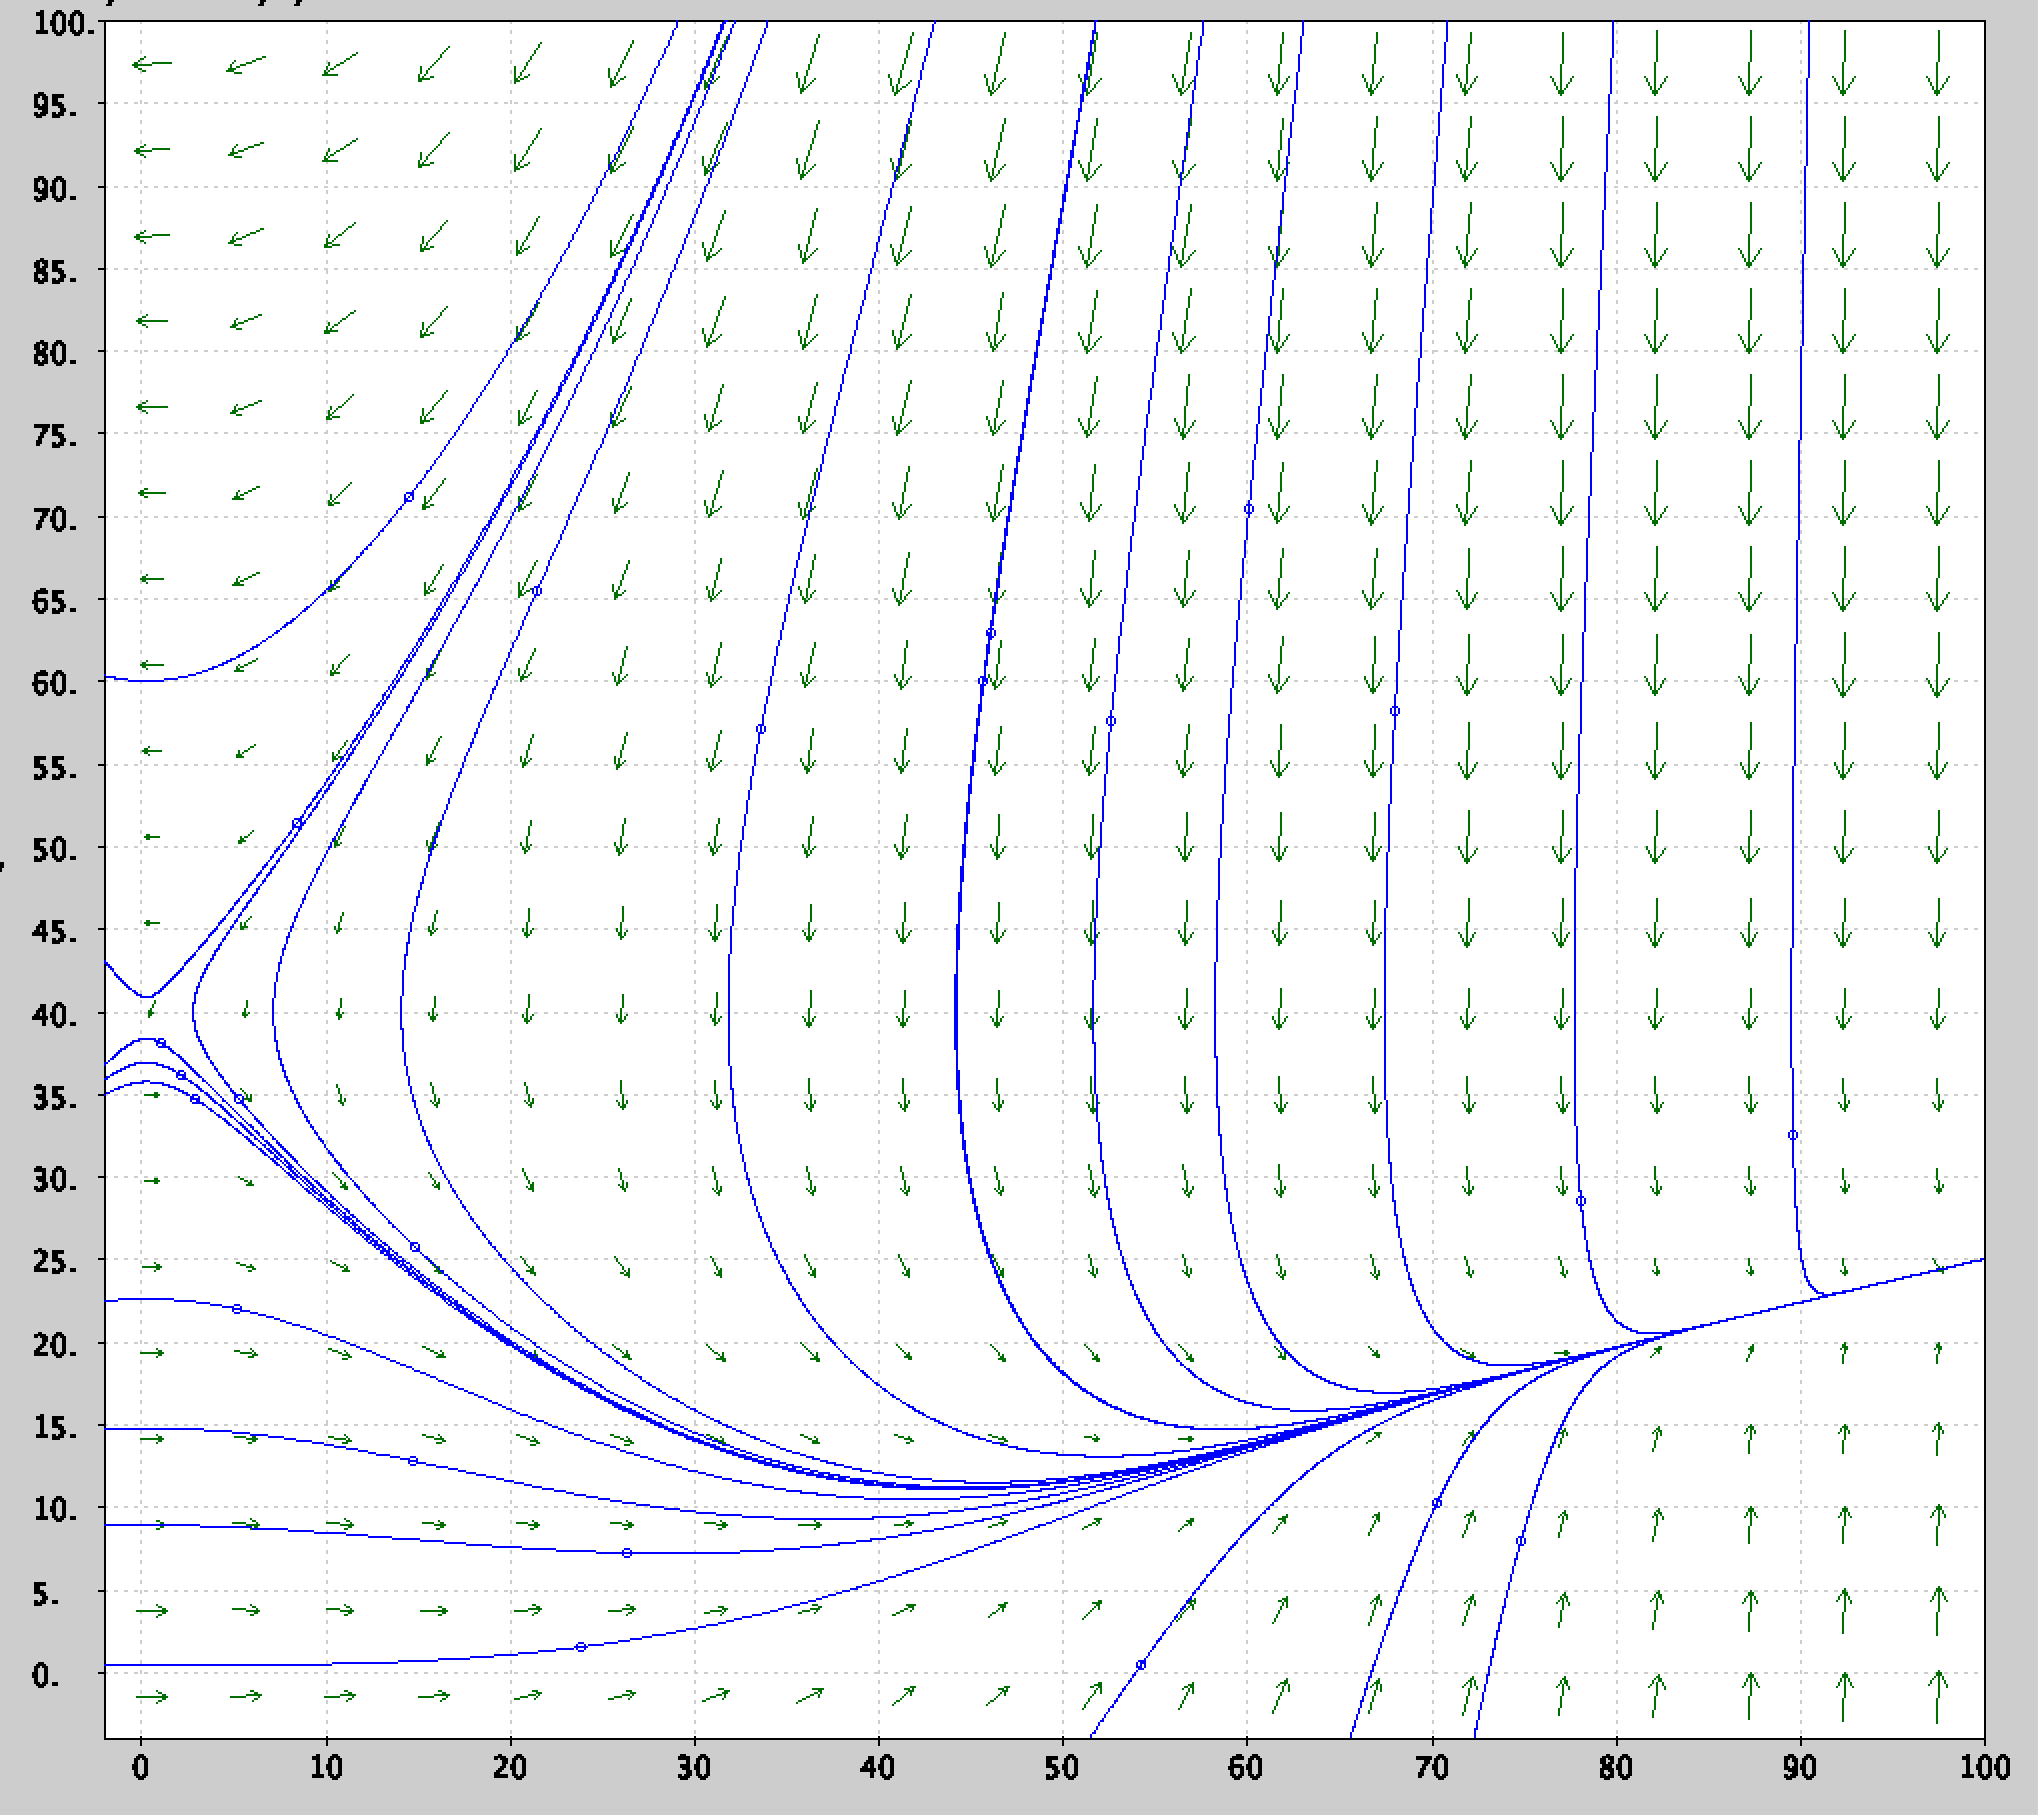
\includegraphics[width=\linewidth]{fig1}
		  \caption{A.}
		  % \label{}
	\endminipage\hfill
		\minipage{0.32\textwidth}
		  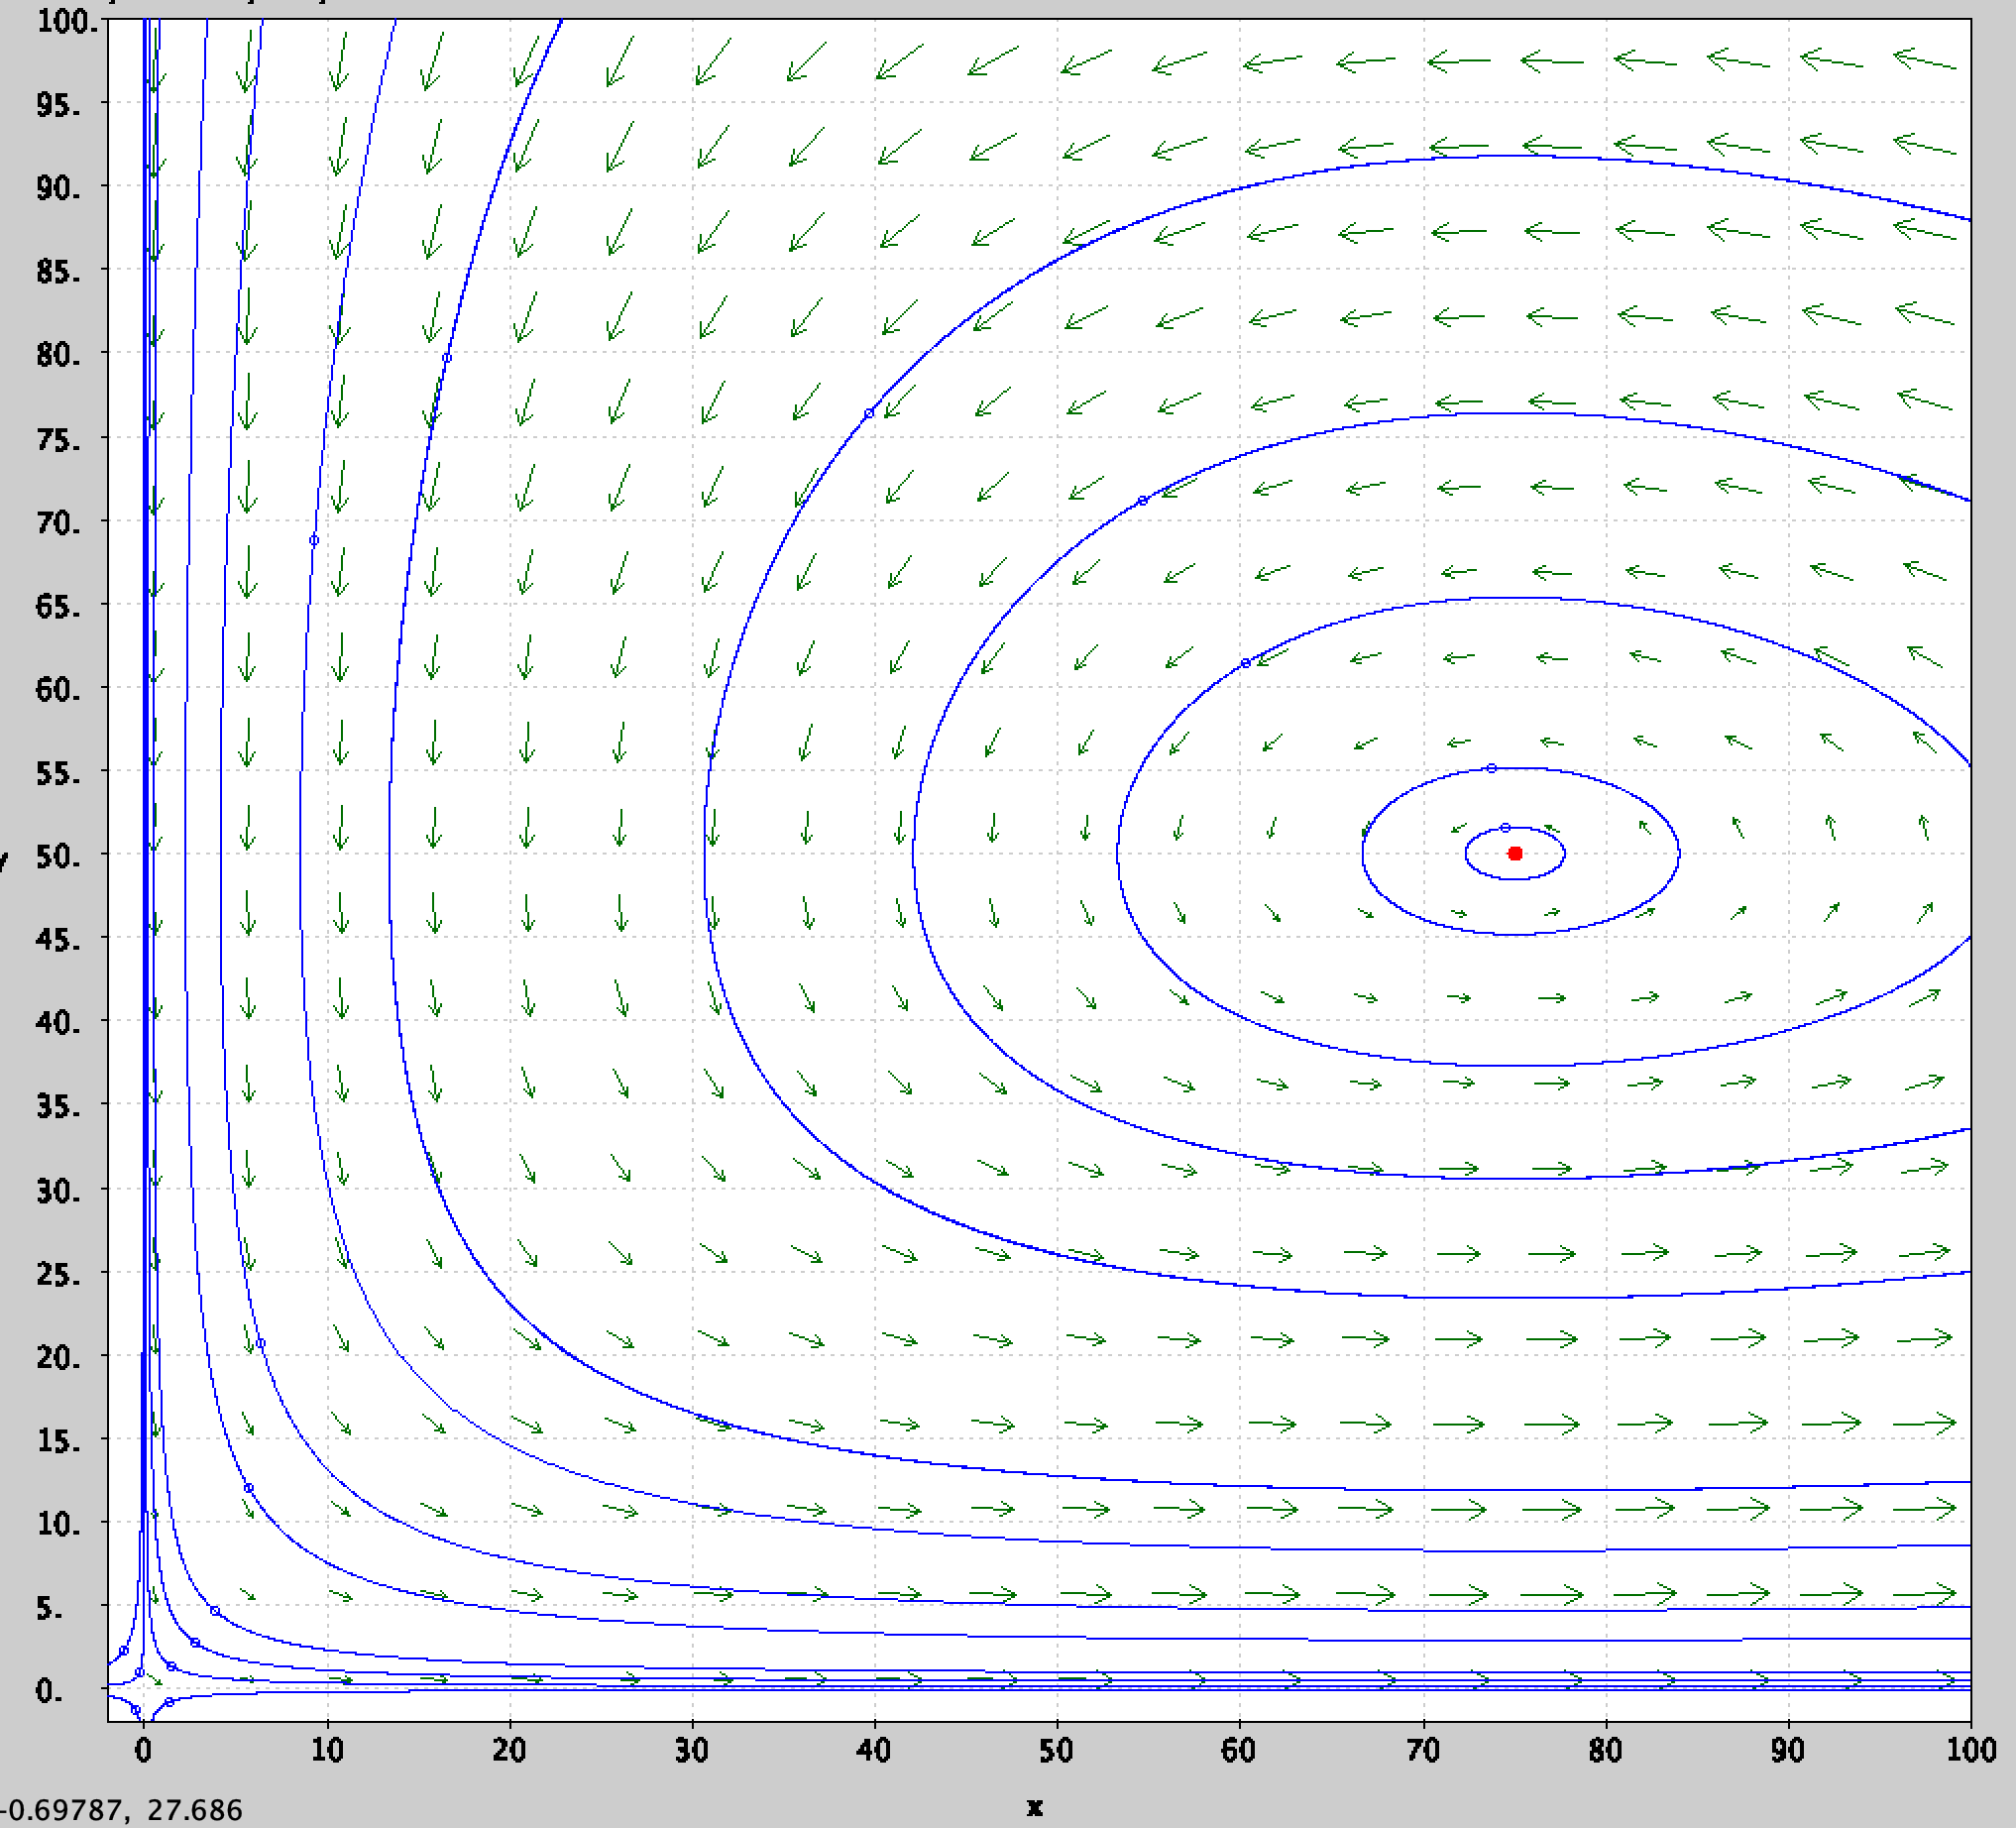
\includegraphics[width=\linewidth]{fig2}
		  \caption{B.}
		  \label{}
	\endminipage\hfill
		\minipage{0.32\textwidth}
		  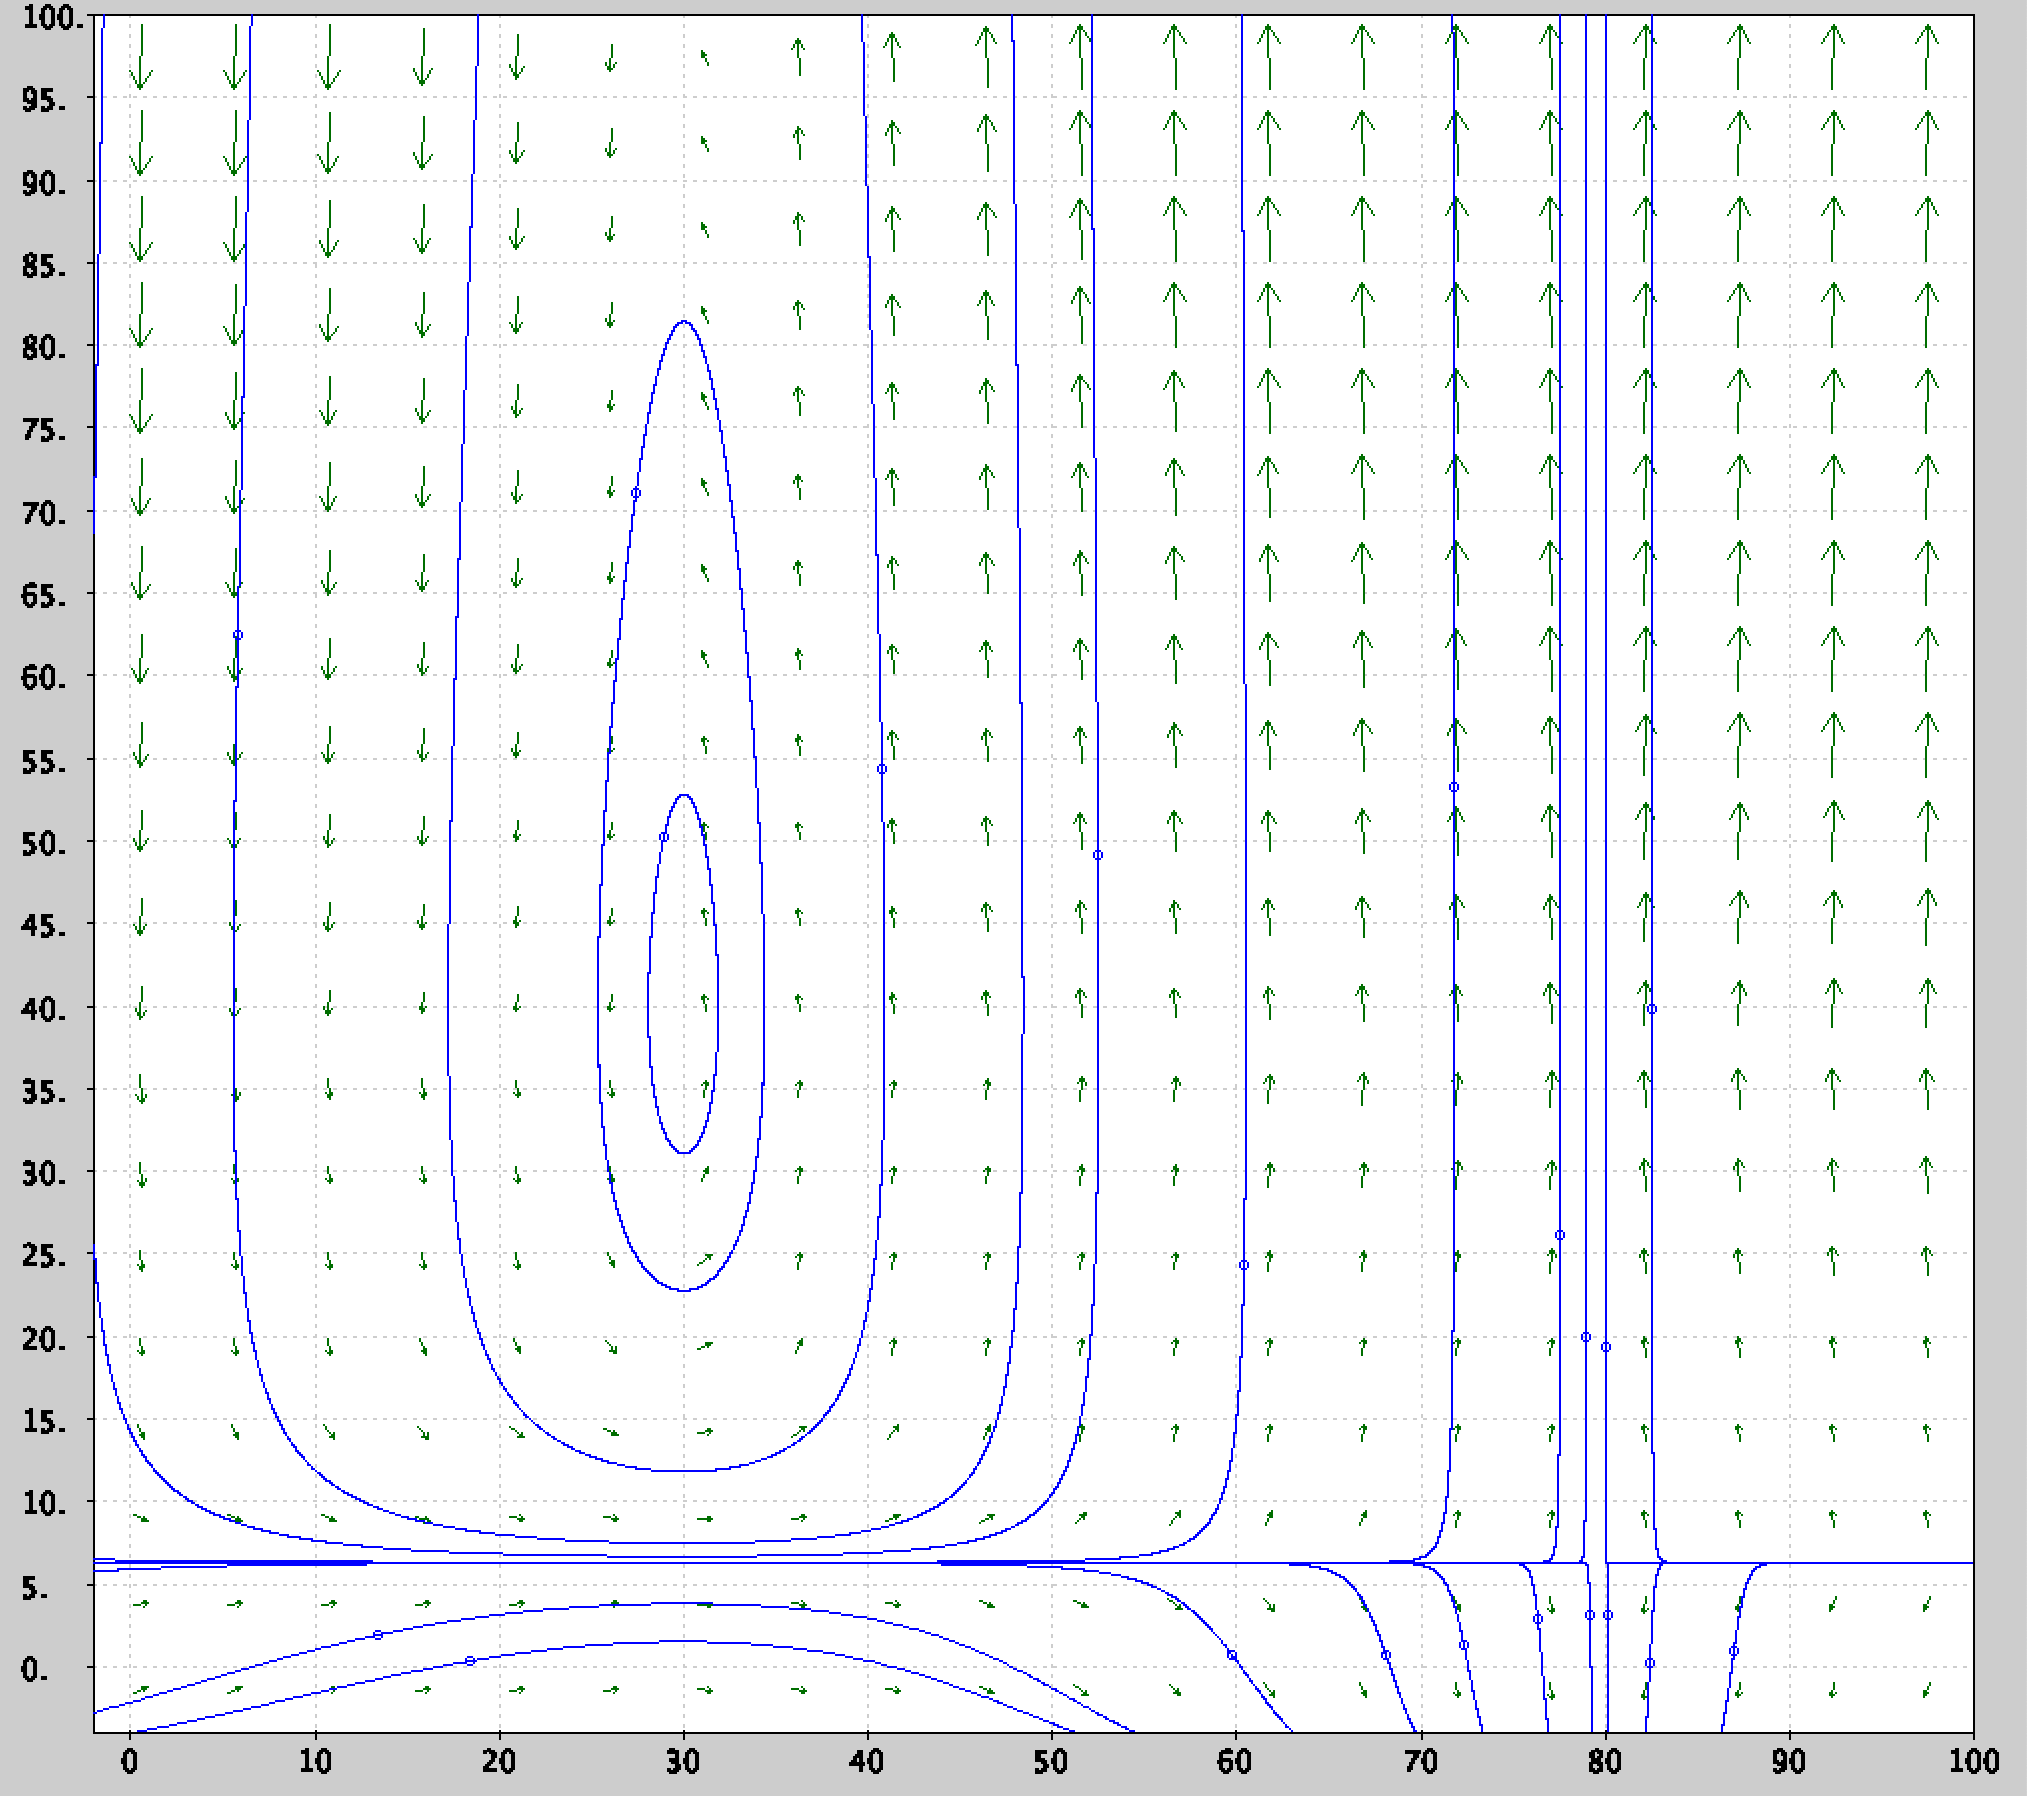
\includegraphics[width=\linewidth]{fig3}
		  \caption{C.}
		  \label{}
		\endminipage
		\end{figure}
		\item Based on the phase plane portrait in part \ref{4}, describe the behavior of the two populations as time evolves, assuming that at time 0 there are 70 rabbits and 45 foxes in the forest. What if we initially have 75 rabbits and 50 foxes?
\end{enumerate}


\subsection*{Logistic Populations}
In this case we have two species with populations $x(t)$ and $y(t)$ which in absence of interaction between them would satisfy logistic equations
\begin{equation}
 		\frac{dx}{dt}=a_1x-b_1x^2,\qquad \frac{dy}{dt}=a_2y-b_2y^2,
\end{equation}
 	with $a_j, b_j>0$, $j=1,2$.
If two such populations interact, this interaction might be beneficial for both of them (i.e. both populations grow as a result of the interaction; \textbf{cooperation}), or it might be beneficial for only one of them while the other is hurt (\textbf{predation}), or it might hurt both of them (\textbf{competition}).
The general form of the system  with (non-trivial) interaction of the two populations is as follows, with $c_1$, $c_2\neq 0$:
\begin{align}
 		\frac{dx}{dt}=a_1x-b_1x^2-c_1xy\\
 		\frac{dy}{dt}=a_2y-b_2y^2-c_2xy
 \end{align}
 The signs of $c_1,$ $c_2$ determine the type of the interaction.
 \begin{enumerate}
 	\item What should be the signs in each of the three cases ({cooperation}, {predation}, {competition})?
 \end{enumerate}
 

\begin{example}
You are given the following system describing two animal populations:
\begin{equation}
	\begin{aligned}\label{system2}
 		\frac{dx}{dt}=60x-4x^2-3xy\\
 		\frac{dy}{dt}=42y-2y^2-3xy
 \end{aligned}	
\end{equation}
\end{example}
\begin{enumerate}
	\item What is the type of interaction between the two populations?
	\item Show that $(6,12)$ is a critical point for the system and compute its linearization there. What is the type of the critical point $(6,12)$ (spiral sink/source, saddle, node etc)?
	\item Use pplane8 to plot a phase plane portrait of \eqref{system2}.  
	What is the long term behavior of the population if initially $x=70$ and $y=68$? What if $x=70$ and $y=69$? 
	Notice the difference just one individual makes! (Also see p. 401 in the textbook).
\end{enumerate}

% competing for the resources available in their environment. Here we assume the following:
% \begin{enumerate}
%  	\item in absence of interaction between the two populations, they both follow logistic models
 	
%  	\item Interaction between the populations results in a decrease of their growth rates which is proportional to $xy$.
%  \end{enumerate} 
%  We have the \textbf{competition system}
%  	\begin{align}
%  		\frac{dx}{dt}=a_1x-b_1x^2-c_1xy=x (a_1-b_1x-c_1y)\\
%  		\frac{dy}{dt}=a_2y-b_2y^2-c_2xy=y (a_2-b_2x-c_2x)
%  	\end{align}
% with $a_j, b_j, c_j>0$, $j=1,2$.

\end{document}